\section{Step 5: Running the three cases}
\label{sec:runs}

\subsection{Steps for one Mach number}

\begin{enumerate}
\item \gui{Initialization}\then\gui{Hybrid}\then\gui{Initialize}. Hybrid initialisation builds a
smooth first guess of the flow around the body from the boundary values, which is a much better start
than a uniform field.
\item First order, CFL 1, for 100 iterations (\gui{Run Calculation}\then\gui{Number of Iterations}\then
\gui{Calculate}, or \texttt{/solve/iterate 100} in the console). Watch \texttt{cd-nose}: it falls
from about 1.3--1.7 (the initial field) as the shock forms.
\item First order, CFL 5, to iteration 400 (density-based). The pressure-based run stays in first order
for 200 iterations, with its automatic pseudo-time step.
\item Switch every equation to second order upwind and iterate until the criterion of
Section~\ref{sec:solver} holds over the last 500 iterations. If the residuals start to grow, lower the
CFL (5\then 3).
\item Save the case and the data (\gui{File}\then\gui{Write}\then\gui{Case \& Data}) with the Mach number
in the name, \file{studyA_M1.47.cas.h5}; save the \texttt{cd-nose} history file under the same name.
\item Read the results: $C_D$ and its pressure/viscous split from \gui{Reports}\then\gui{Forces} on
\zone{wall\_nose}; the maximum $y^+$ on both walls from \gui{Reports}\then\gui{Surface Integrals} or a
contour of \gui{Wall Yplus}; Mach contours for the flow field (Section~\ref{sec:results}).
\end{enumerate}

\paragraph{Next Mach number.} Read the converged case, change $p_\infty$, $M$ and $T_\infty$ on
\zone{inlet} and \zone{farfield}, $p_\infty$ and the backflow temperature on \zone{outlet} (the
turbulence values follow from $I$ and $\mu_t/\mu$), redo \gui{Reference Values}\then\gui{Compute from}
\zone{inlet}, and \textbf{initialise again} before step~2.
Restarting $M = 1.2$ from the $M = 1.47$ solution went unstable after 180 iterations: the bow shock has to
move too far. A fresh hybrid initialisation also resets the iteration count and the plots.

\checkstep{Before calling a run converged: $\Delta < 0.1\,\%$ over the last 500 iterations, the
maximum $y^+$ is below 1, and $C_D$ recomputed from the force equals the reported value.}

\subsection{The runs of study A}

\begin{table}[H]
\centering
\caption{Run history. $\Delta$ is the $C_D$ variation over the last 500 iterations.}
\label{tab:runs}
\small
\begin{tabularx}{\linewidth}{@{}llll>{\raggedright\arraybackslash}X@{}}
\toprule
Run & Iterations & Order & Time step & Note \\
\midrule
$M = 1.47$, density-based & 1--100 & first & CFL 1 & start from hybrid initialisation \\
 & 101--400 & first & CFL 5 & \\
 & 401--3000 & second & CFL 5 & $\Delta = 0.032\,\%$ over 2501--3000 \\
\midrule
$M = 1.2$, density-based & 1--100 & first & CFL 1 & fresh initialisation \\
 & 101--400 & first & CFL 5 & \\
 & 401--2400 & second & CFL 5 & continuity residual rose from $1.3\cdot10^{-3}$ to $8\cdot10^{-3}$ \\
 & 2401--3200 & second & CFL 3 & residuals flat; $\Delta = 0.083\,\%$ over 2701--3200 \\
\midrule
$M = 0.95$, pressure-based & 1--200 & first & pseudo-time & $C_D$ steady at 0.0488 \\
 & 201--1200 & second & pseudo-time & $\Delta = 0.009\,\%$ over 701--1200 \\
\midrule
$M = 0.95$, density-based & 1--4300 & first, then second & CFL 1--3 & not converged, not used \\
\bottomrule
\end{tabularx}
\end{table}

\begin{figure}[H]
\centering
\begin{subfigure}[t]{0.49\linewidth}
\centering
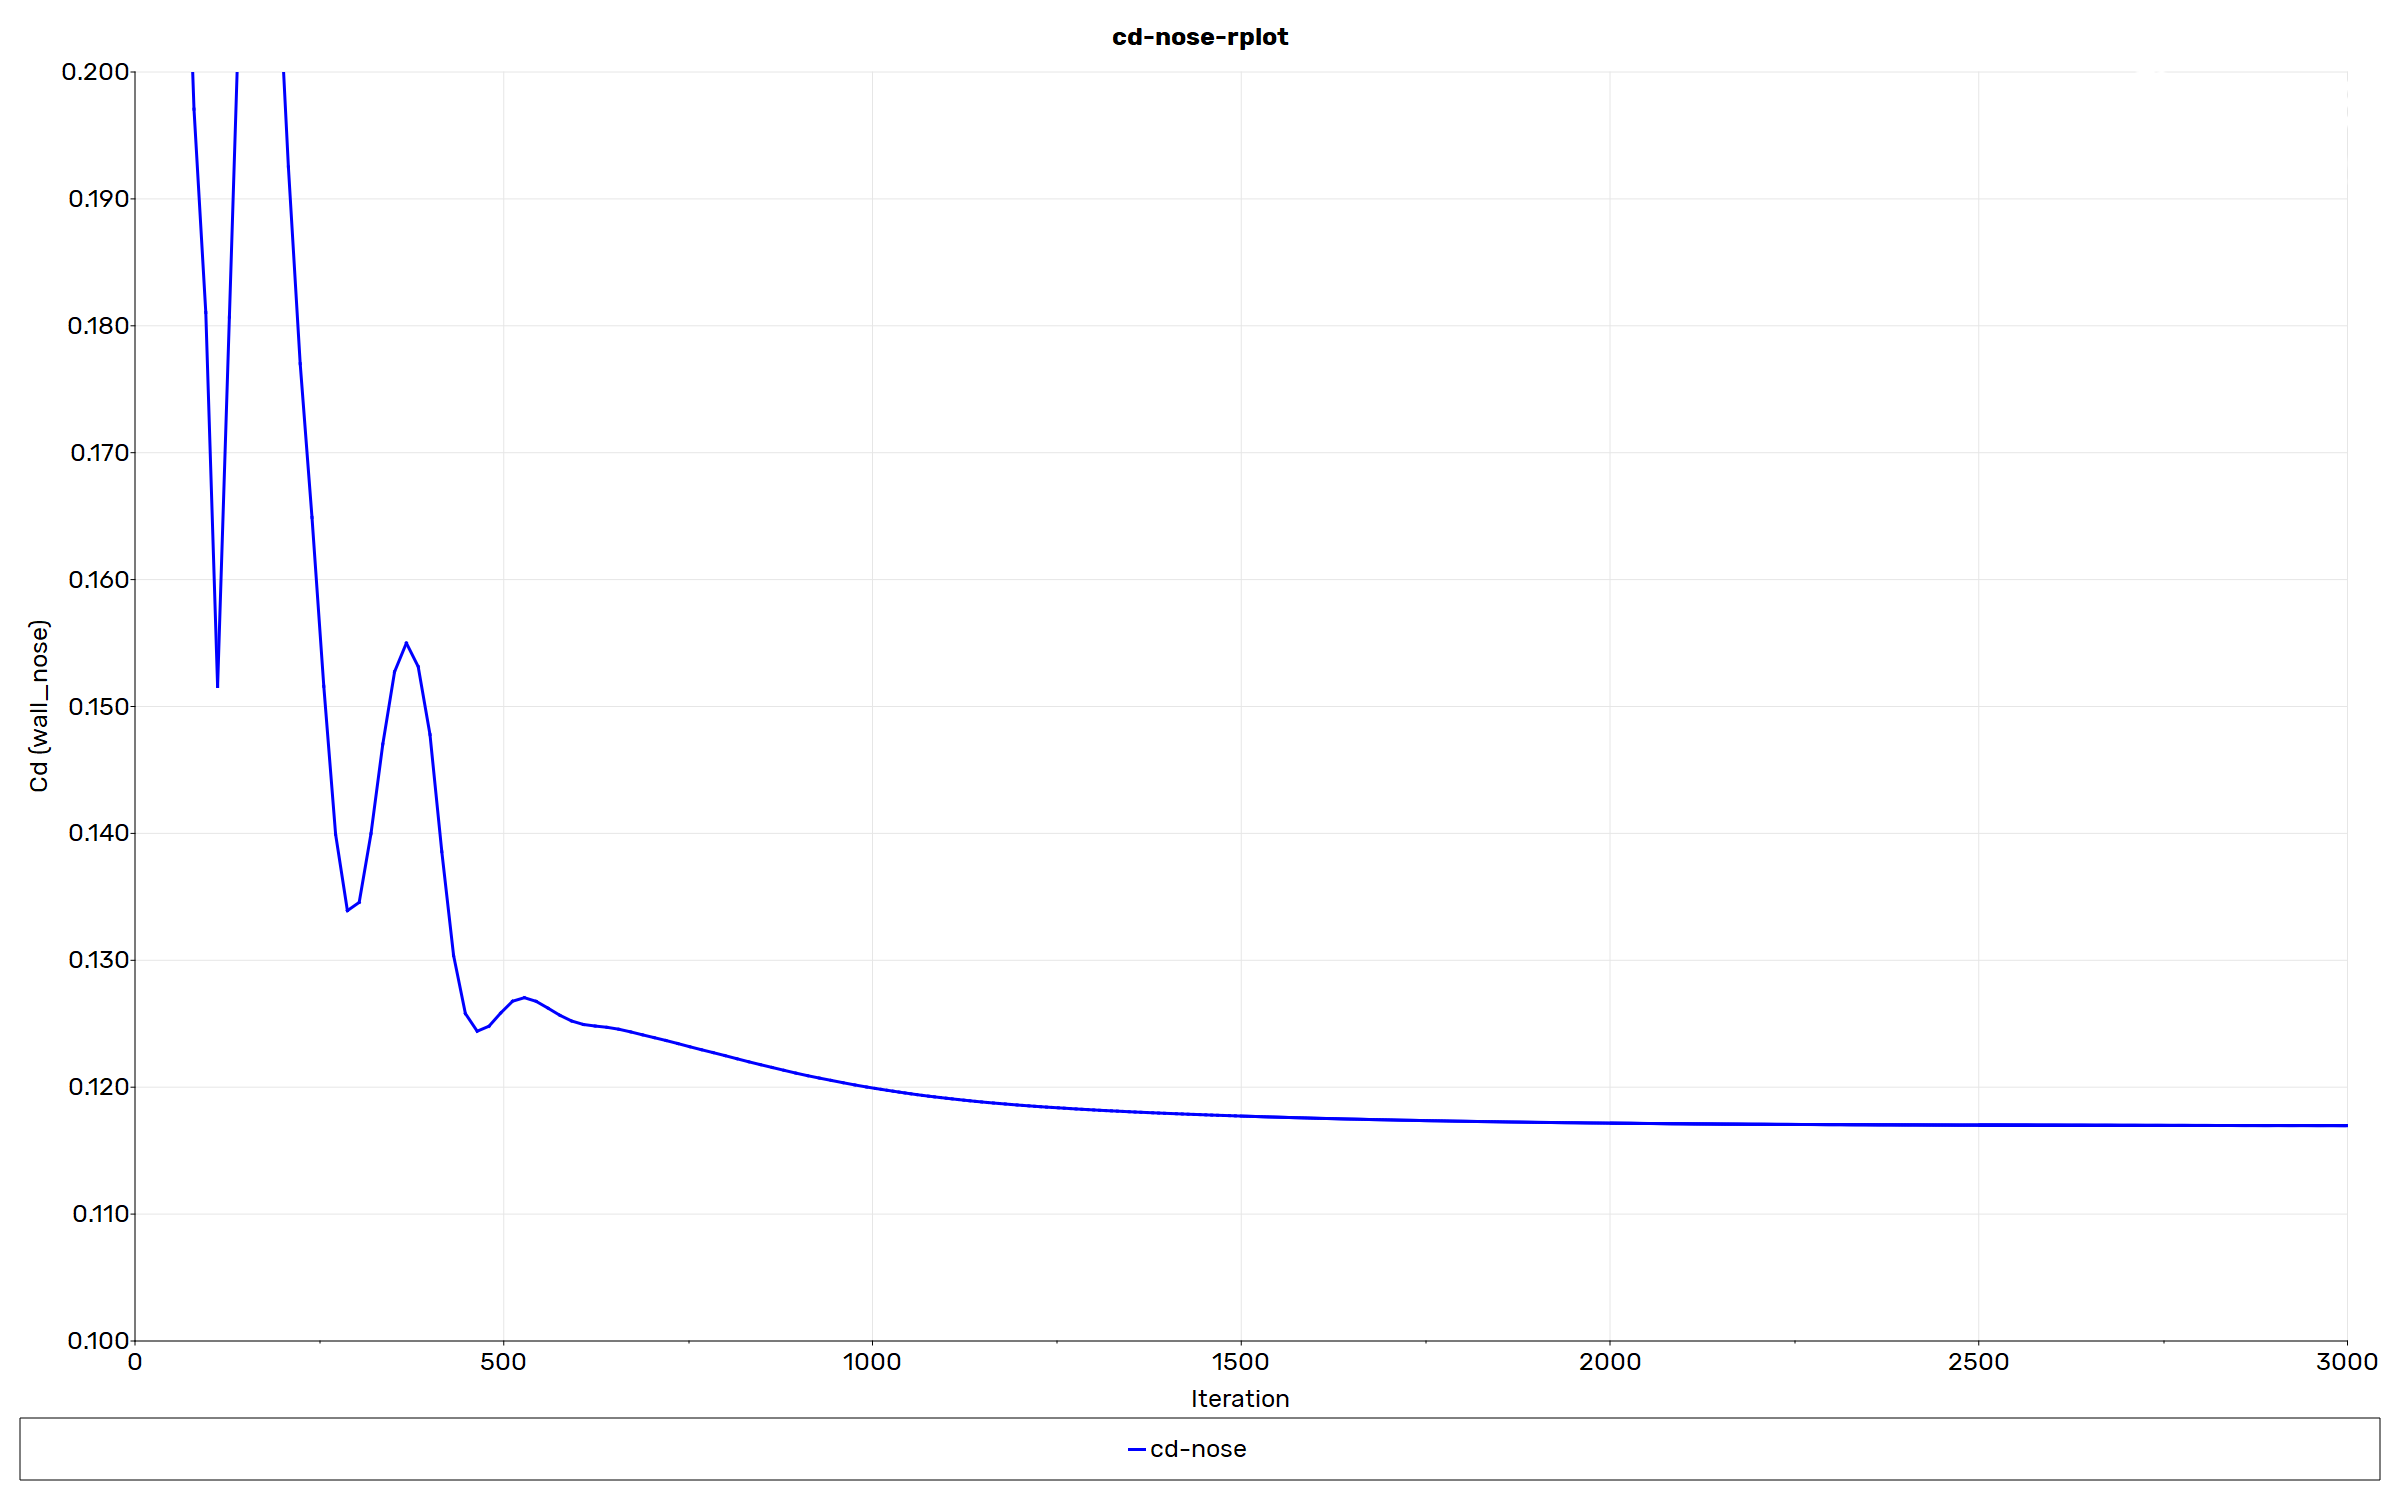
\includegraphics[width=\linewidth]{fluent_cd_M1.47}
\caption{$M = 1.47$, density-based.}
\end{subfigure}\hfill
\begin{subfigure}[t]{0.49\linewidth}
\centering
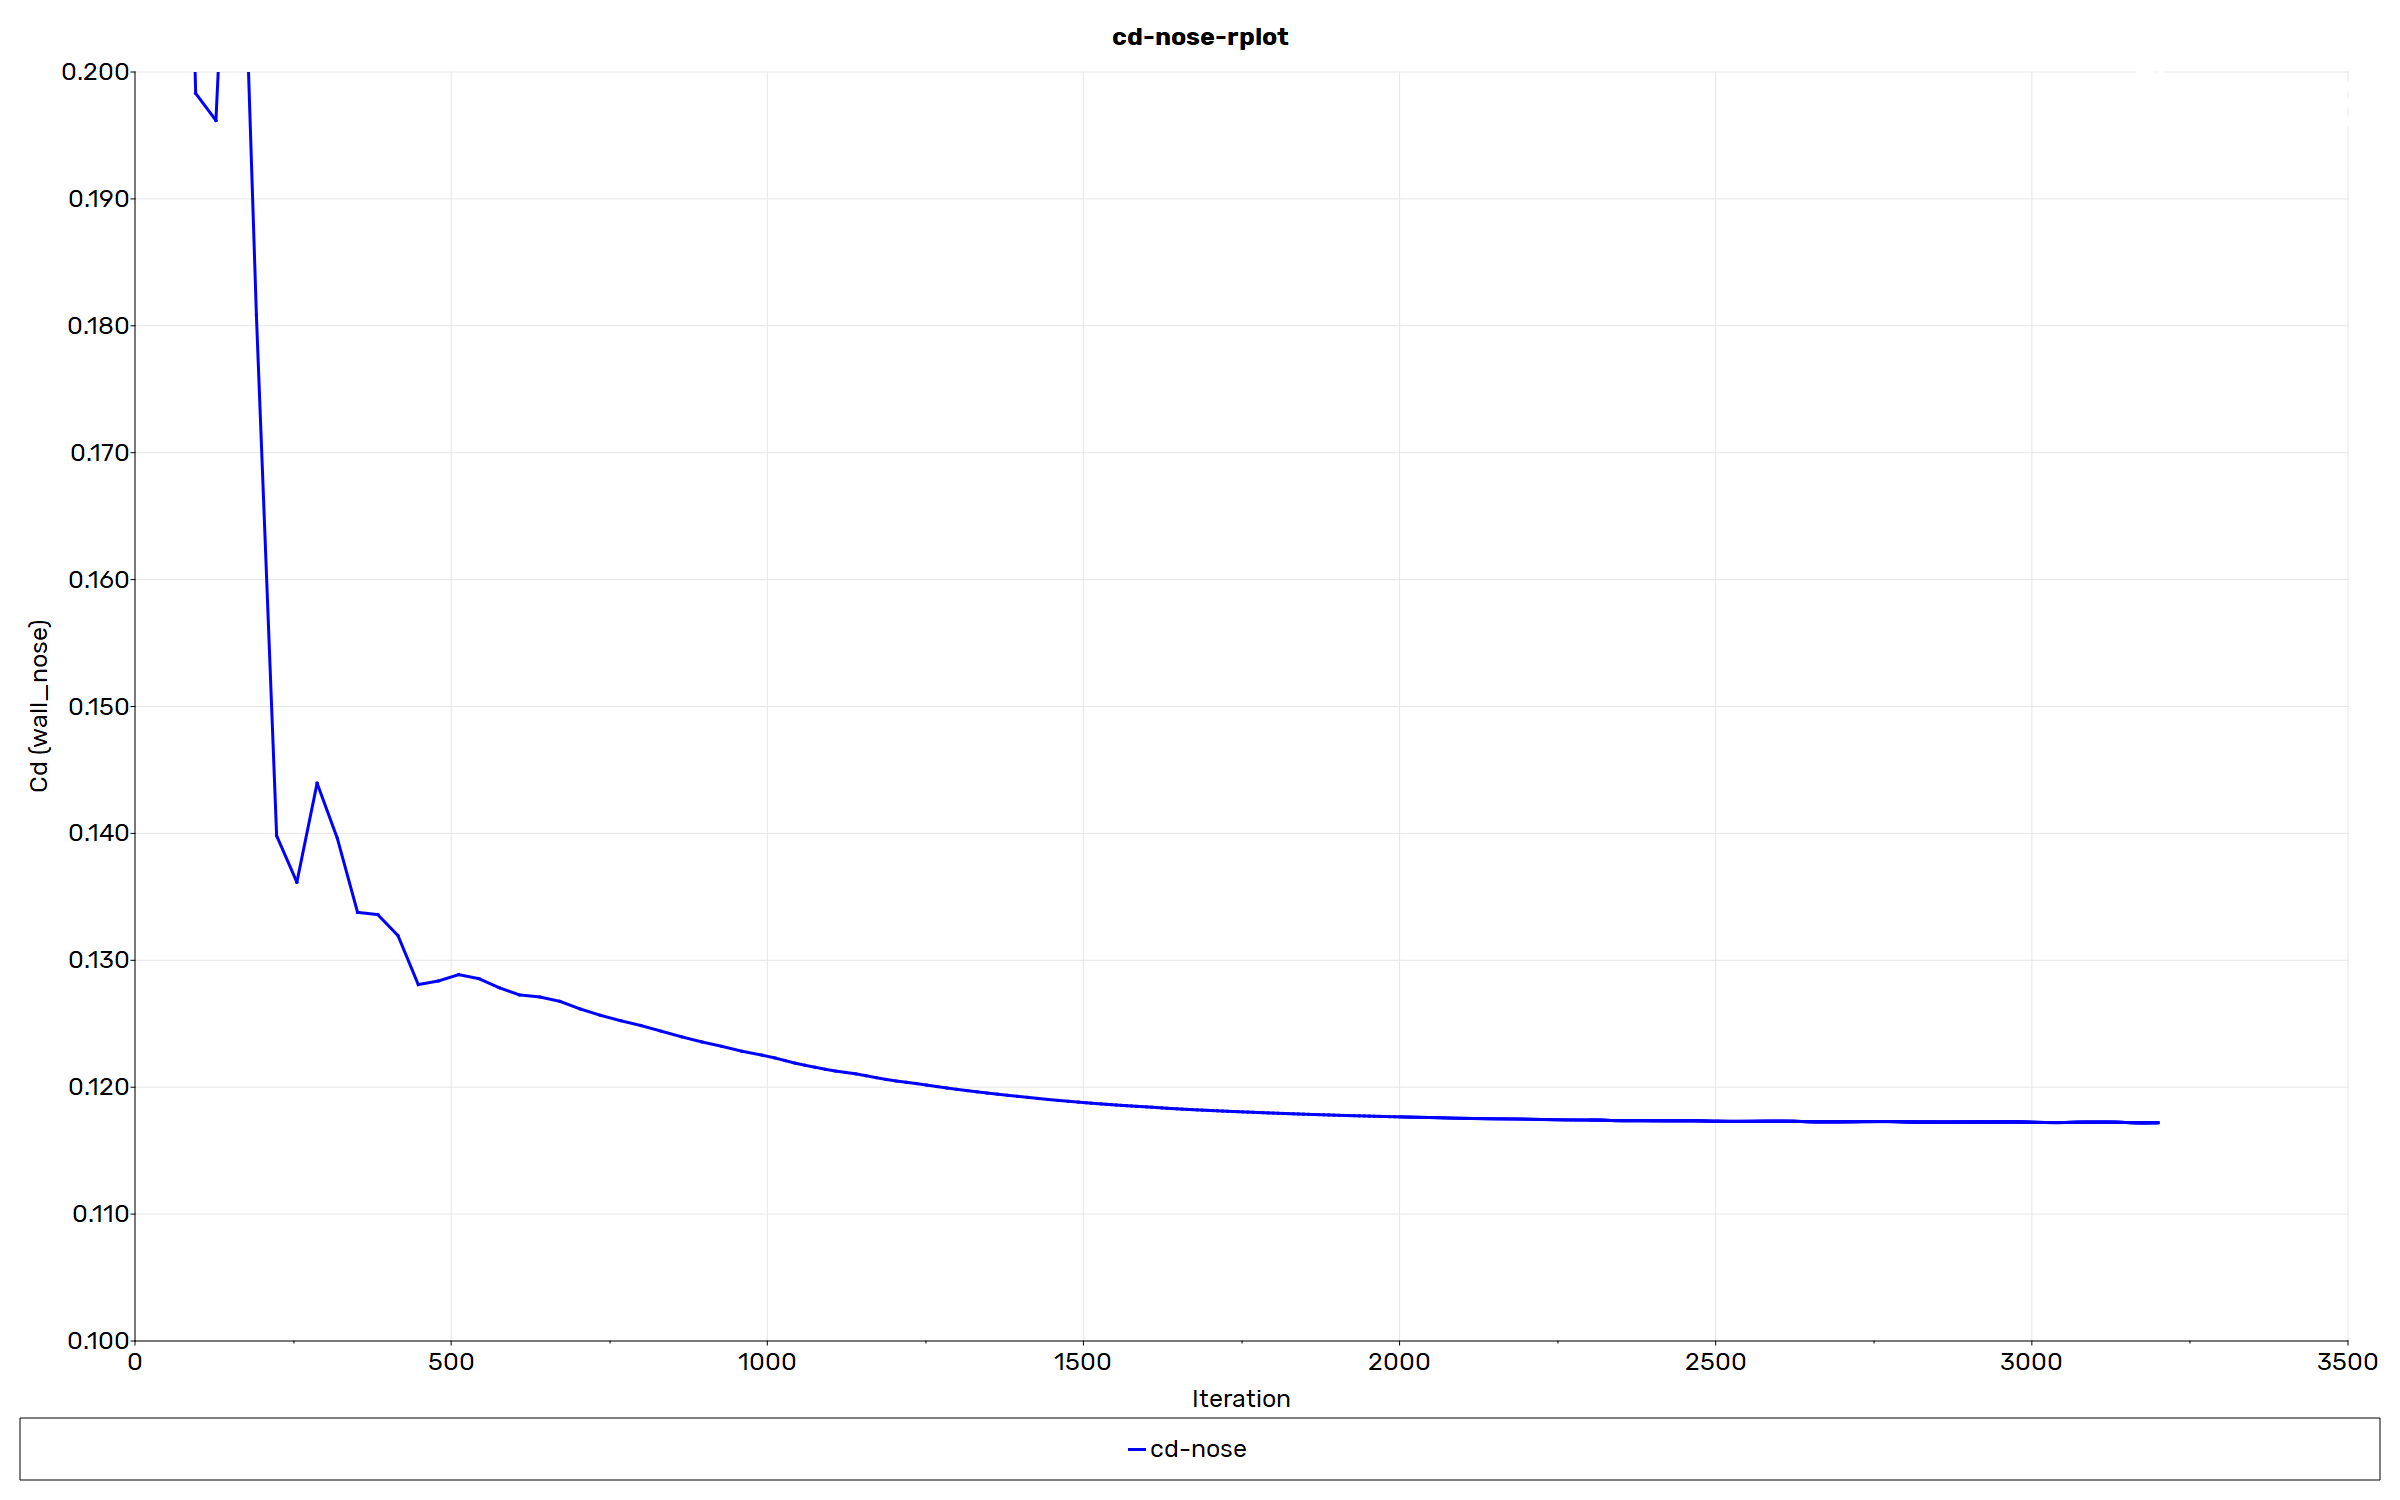
\includegraphics[width=\linewidth]{fluent_cd_M1.20}
\caption{$M = 1.2$, density-based.}
\end{subfigure}

\medskip
\begin{subfigure}[t]{0.49\linewidth}
\centering
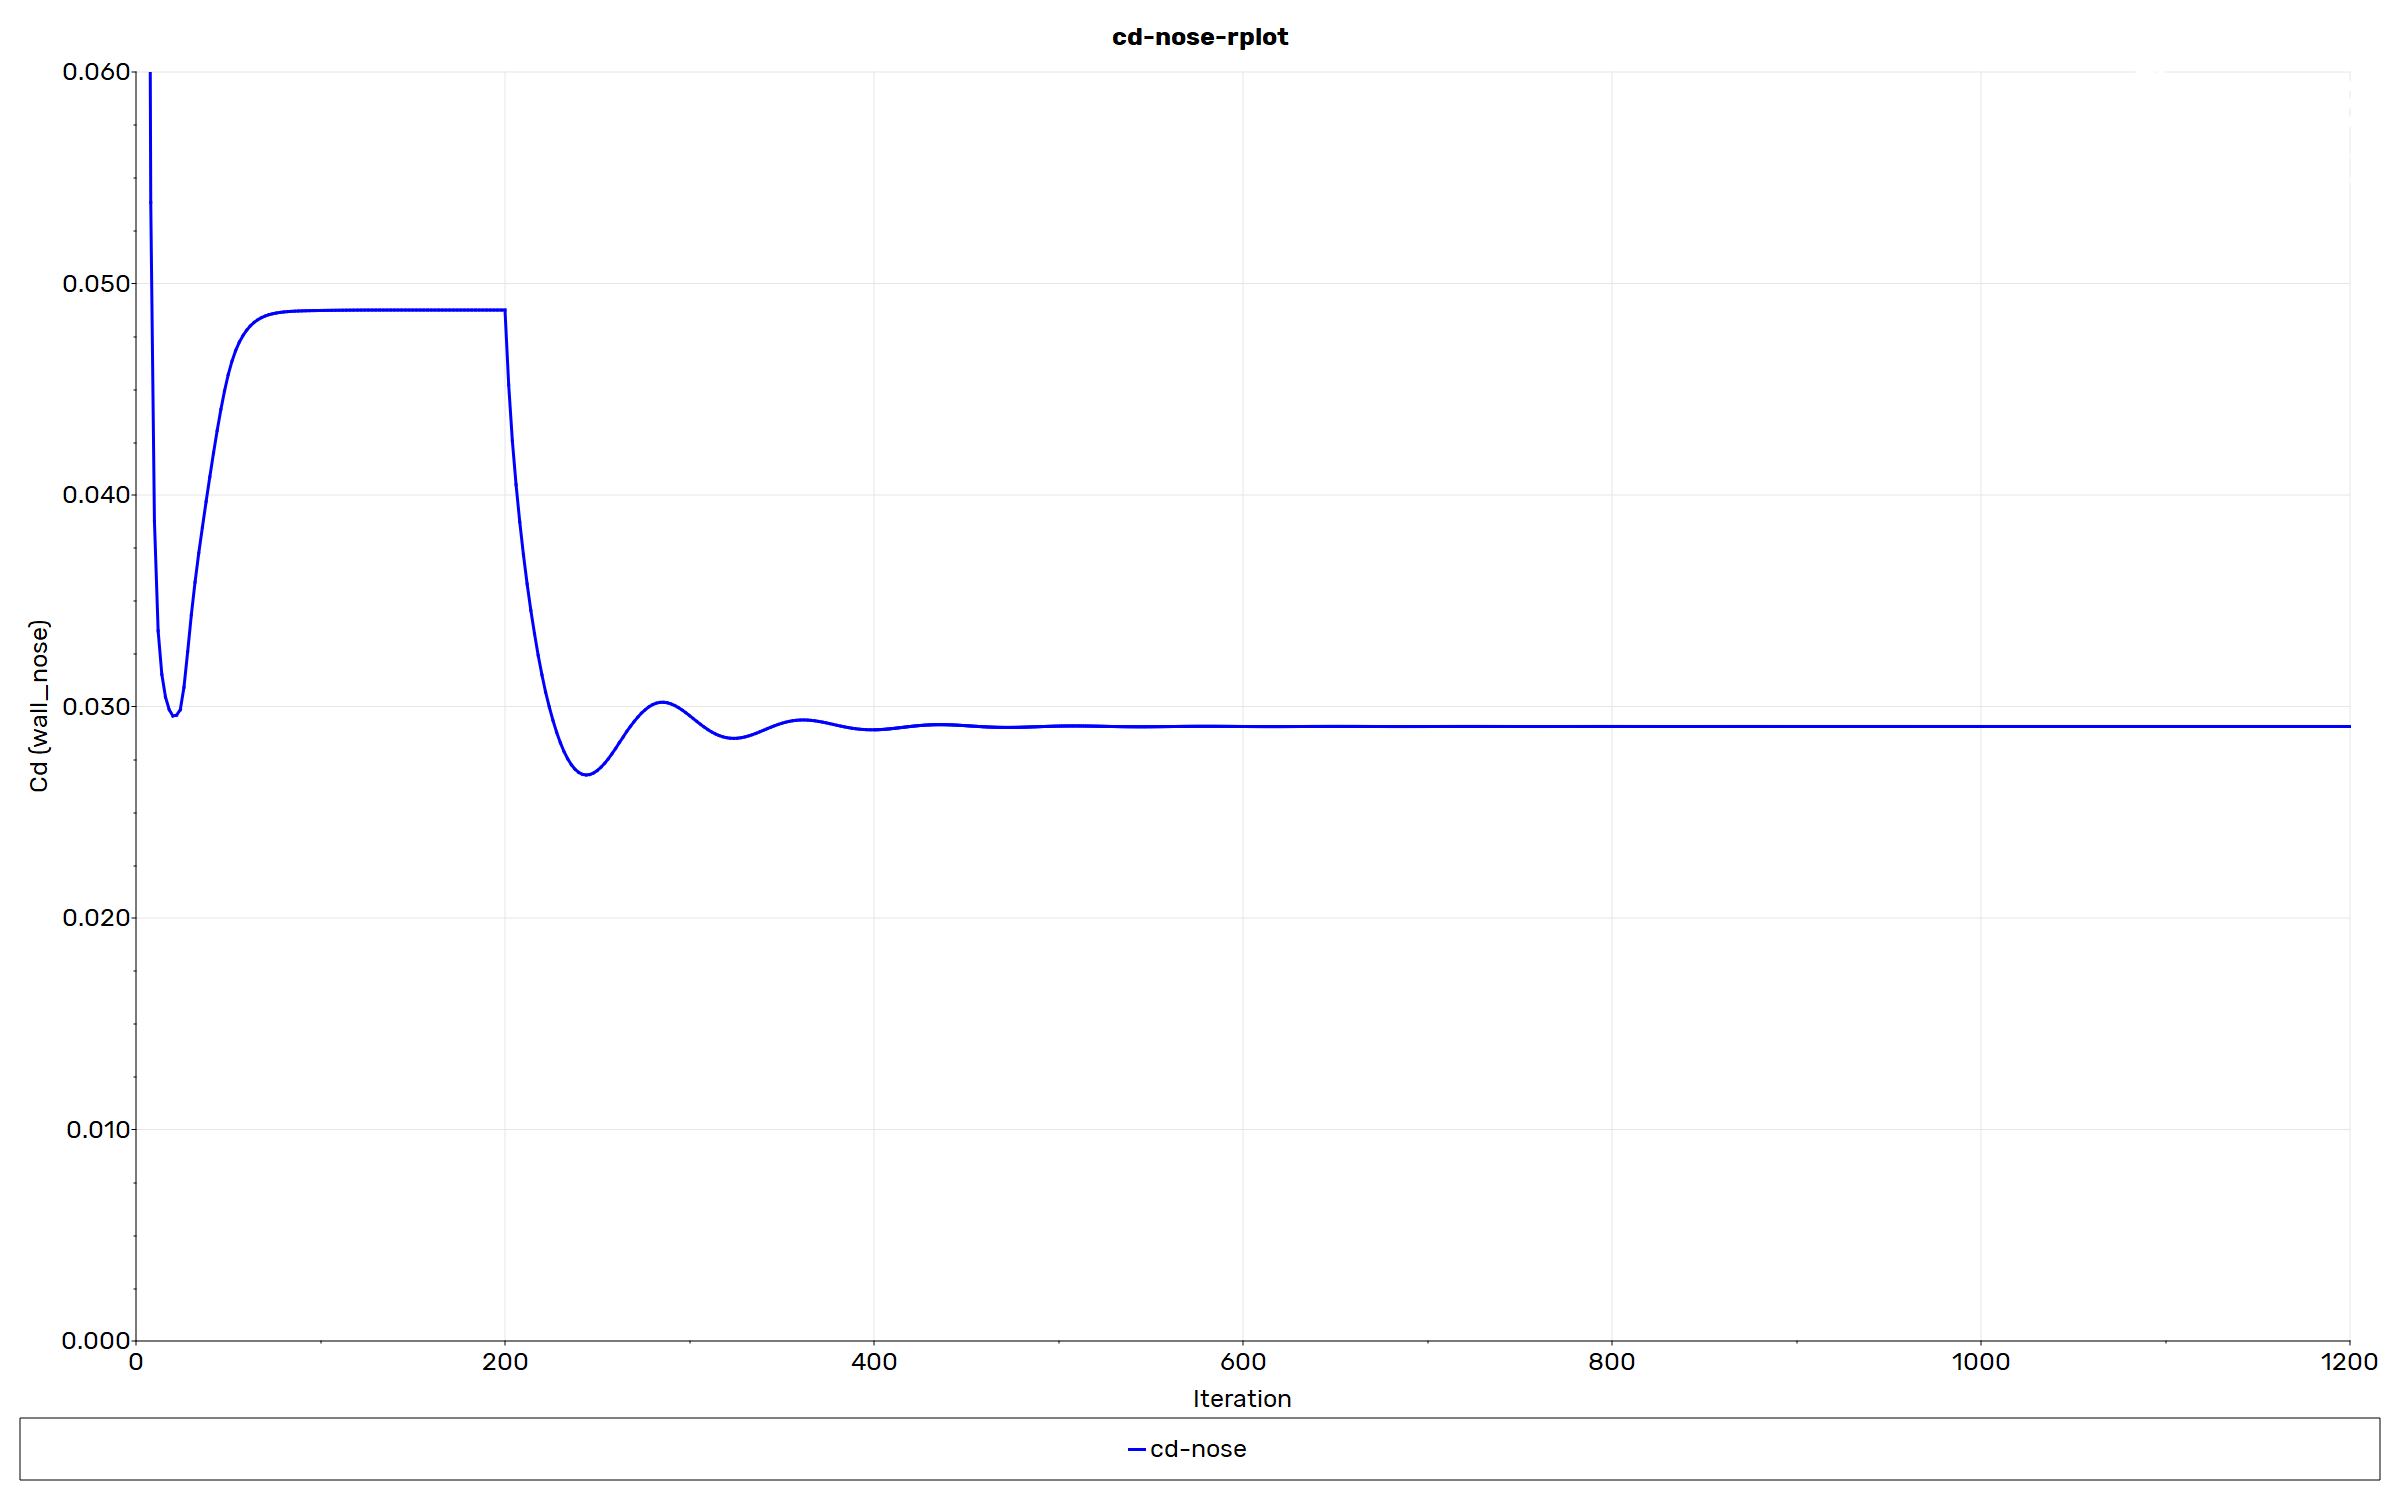
\includegraphics[width=\linewidth]{fluent_cd_M0.95}
\caption{$M = 0.95$, pressure-based.}
\end{subfigure}
\caption{The \texttt{cd-nose} monitor of the three converged runs (Fluent report plots). The vertical
axis is fixed (0.10--0.20 above $M = 1$, 0--0.06 at $M = 0.95$), so the first iterations go off the top.
Second order starts at iteration 400 in (a) and (b) and at iteration 200 in (c).}
\label{fig:history}
\end{figure}

Each curve shows a first-order transient, a drop at the switch to second order (first order adds numerical
dissipation, seen as extra drag), then a slow decay; the last per cent takes 1500--2000 iterations.
First-order values, such as 0.0488 at $M = 0.95$, are only starting fields.

\begin{figure}[H]
\centering
\begin{subfigure}[t]{0.49\linewidth}
\centering
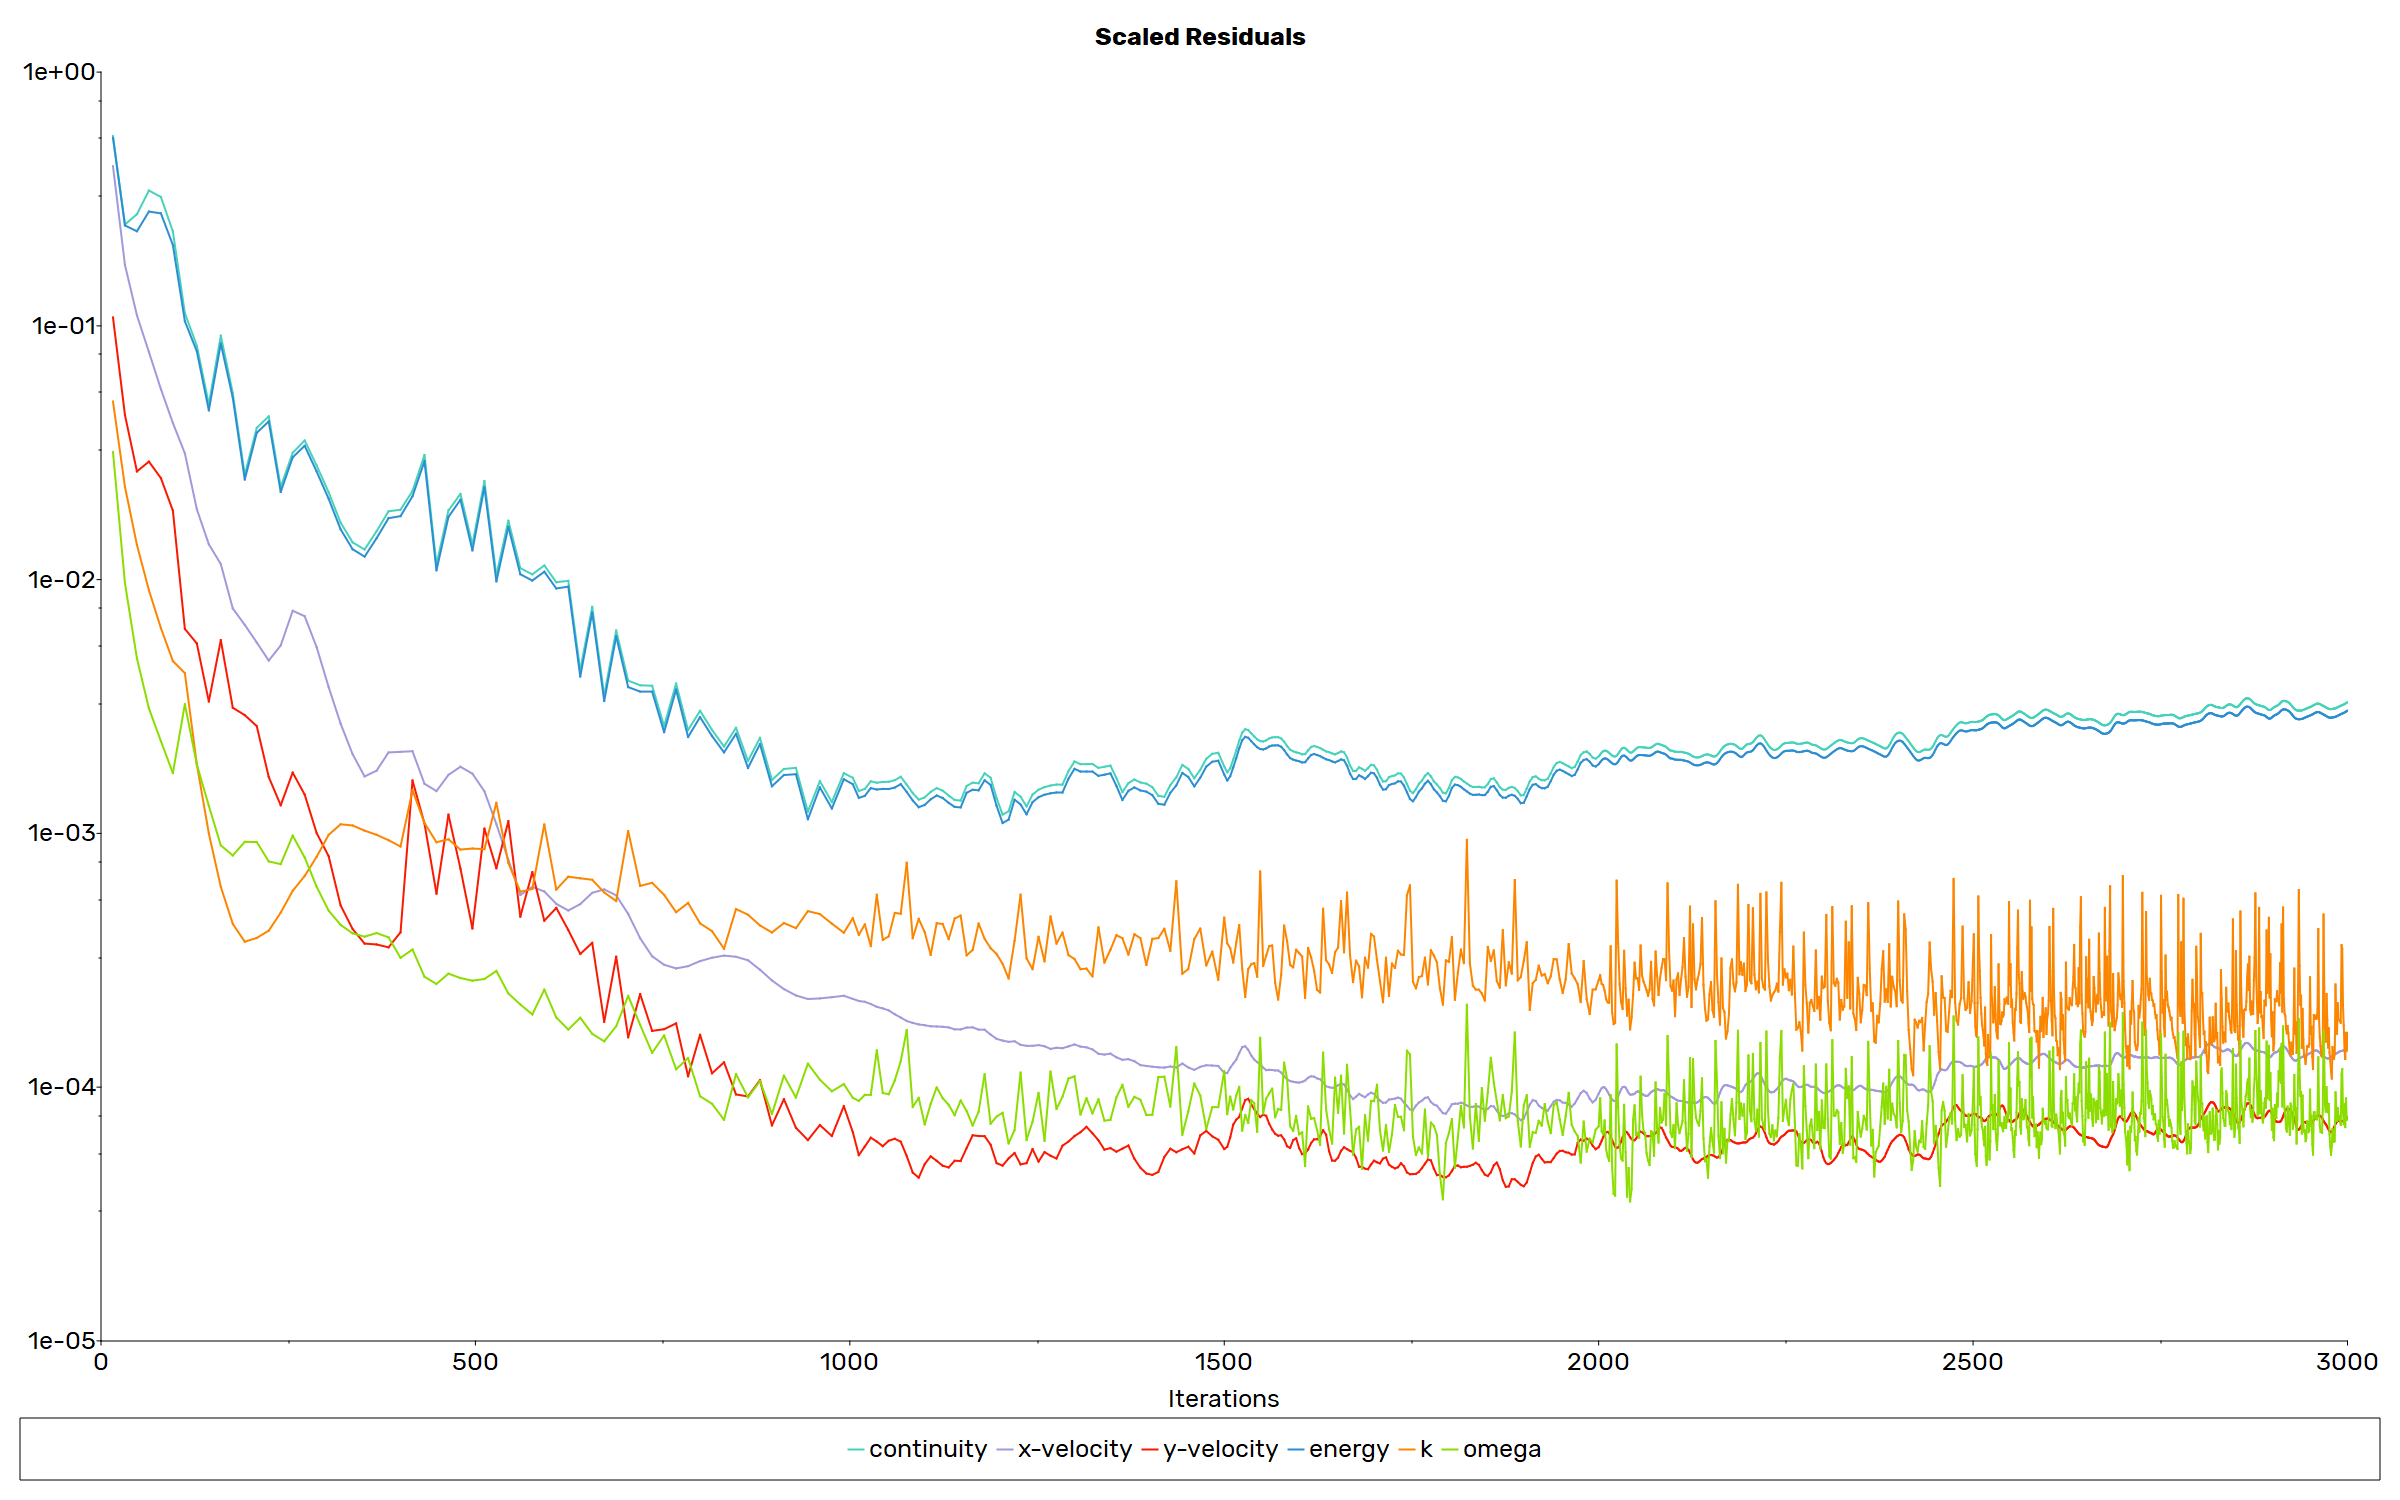
\includegraphics[width=\linewidth]{fluent_residuals_M1.47}
\caption{$M = 1.47$, density-based.}
\end{subfigure}\hfill
\begin{subfigure}[t]{0.49\linewidth}
\centering
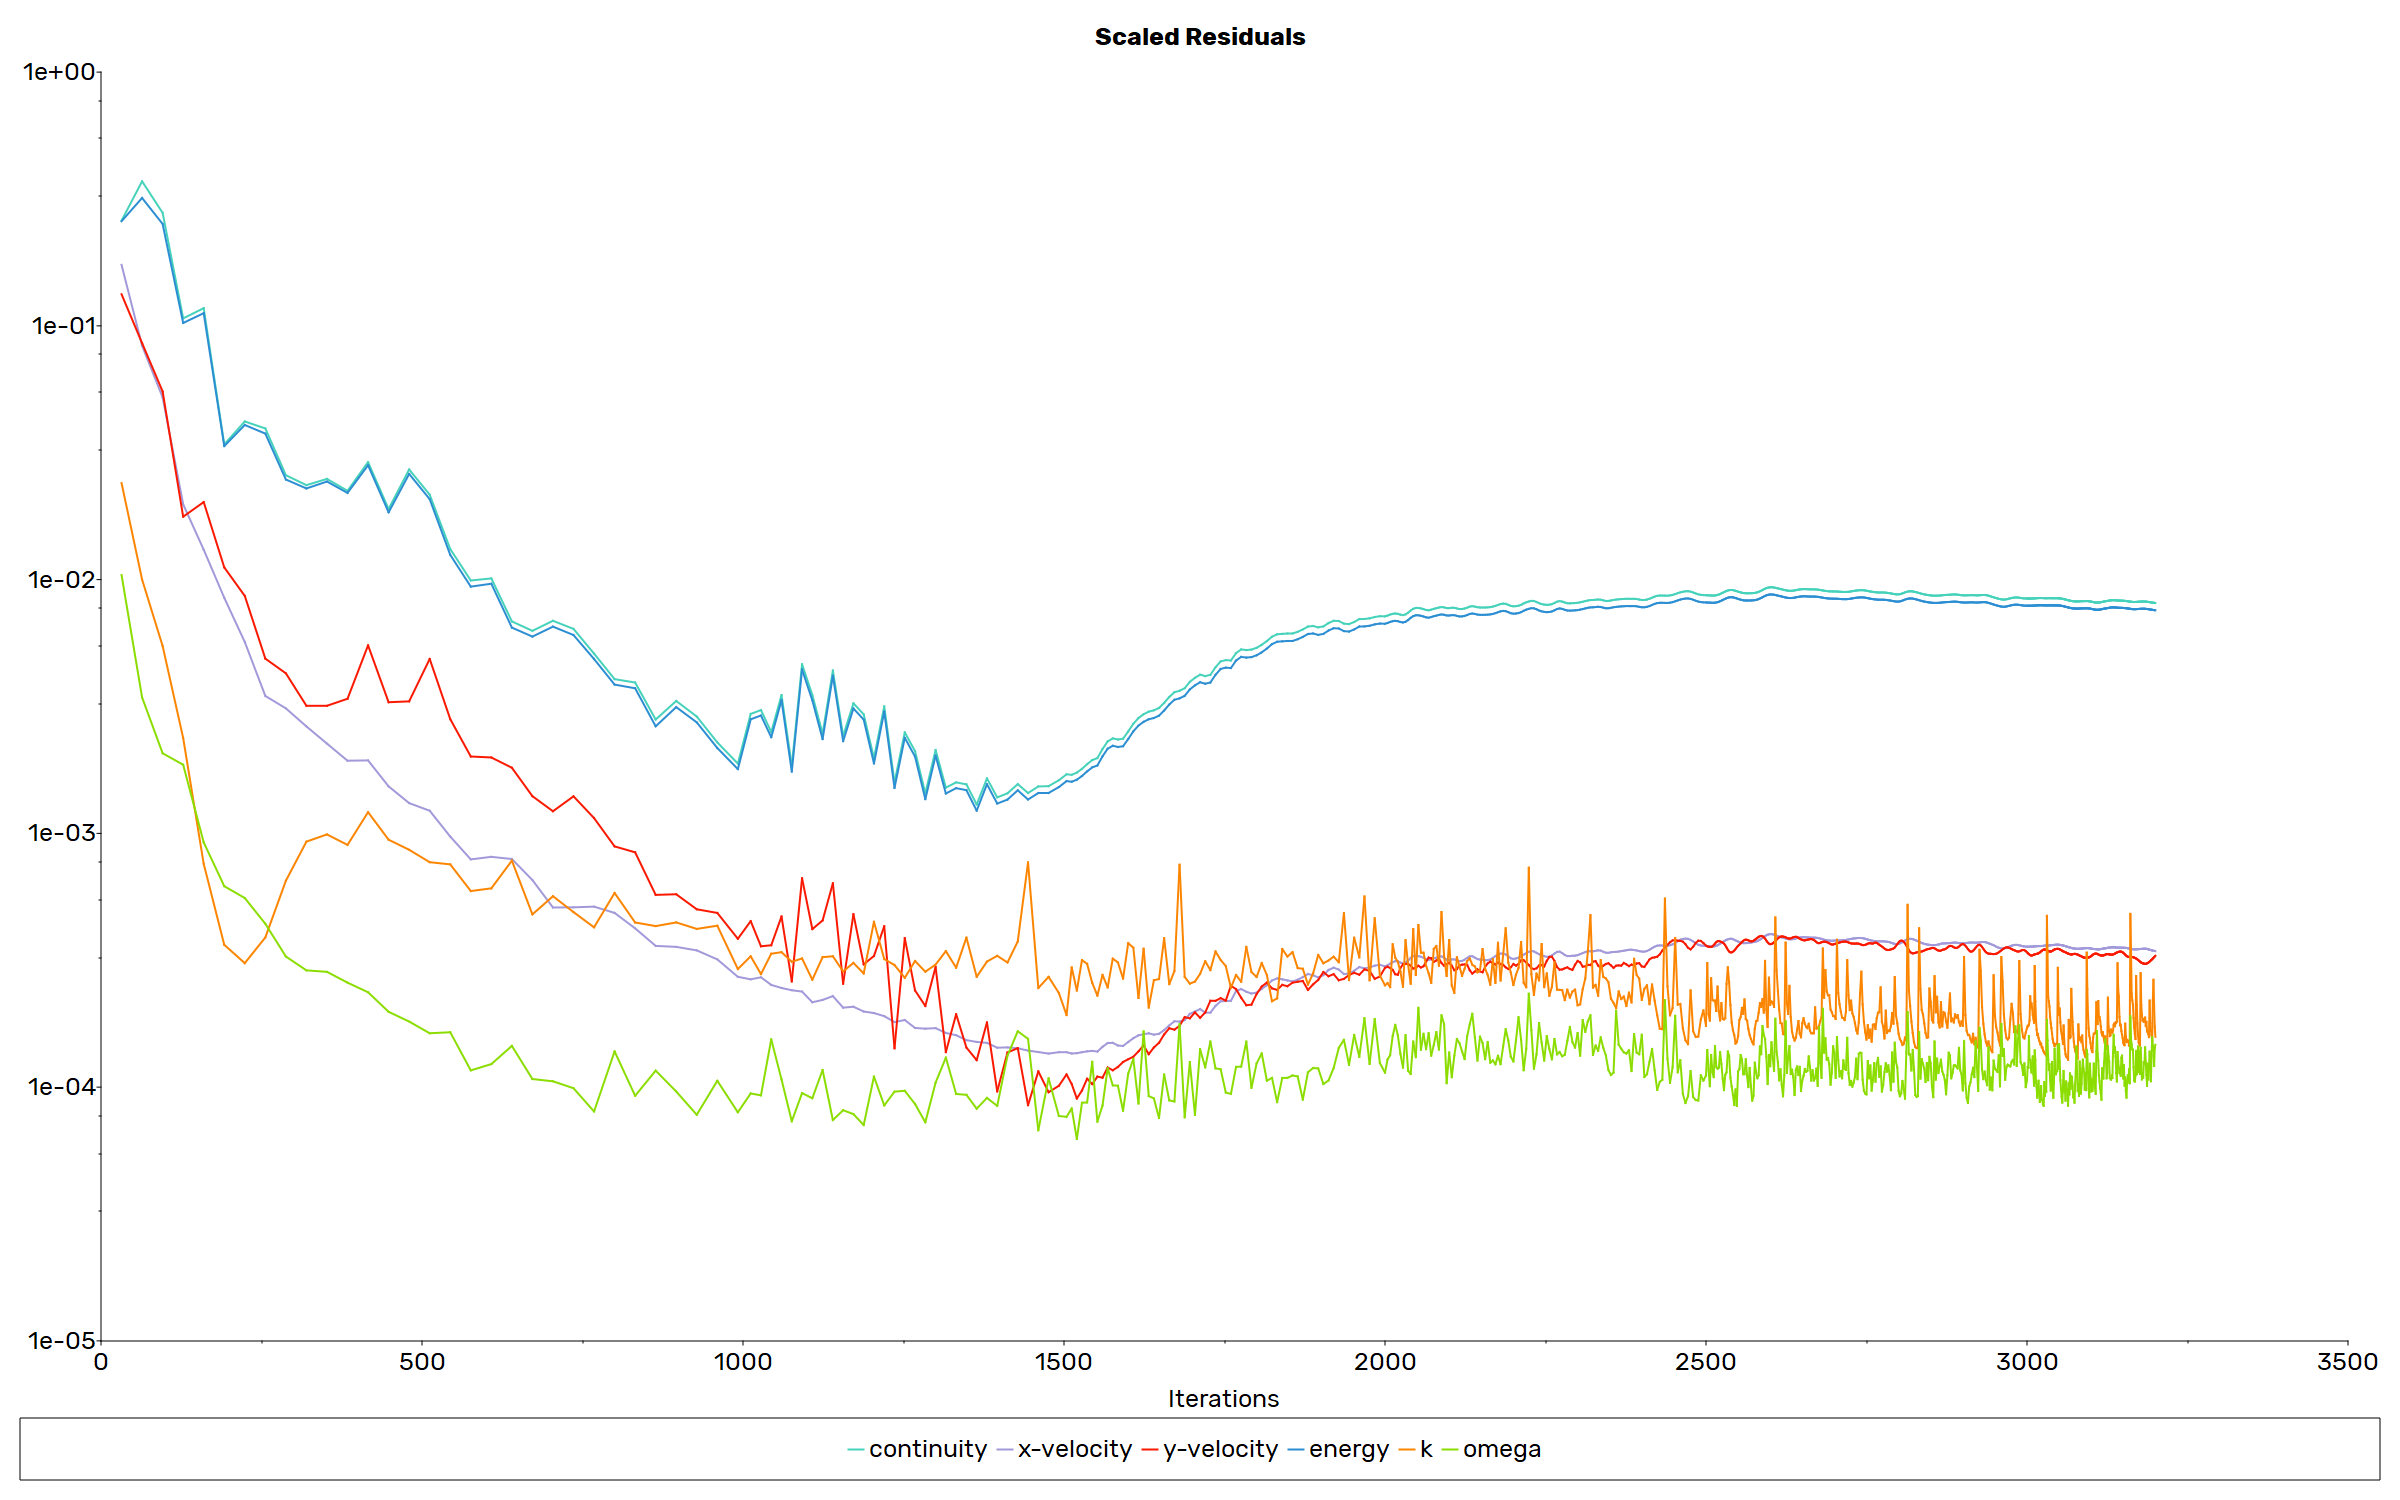
\includegraphics[width=\linewidth]{fluent_residuals_M1.20}
\caption{$M = 1.2$, density-based.}
\end{subfigure}

\medskip
\begin{subfigure}[t]{0.49\linewidth}
\centering
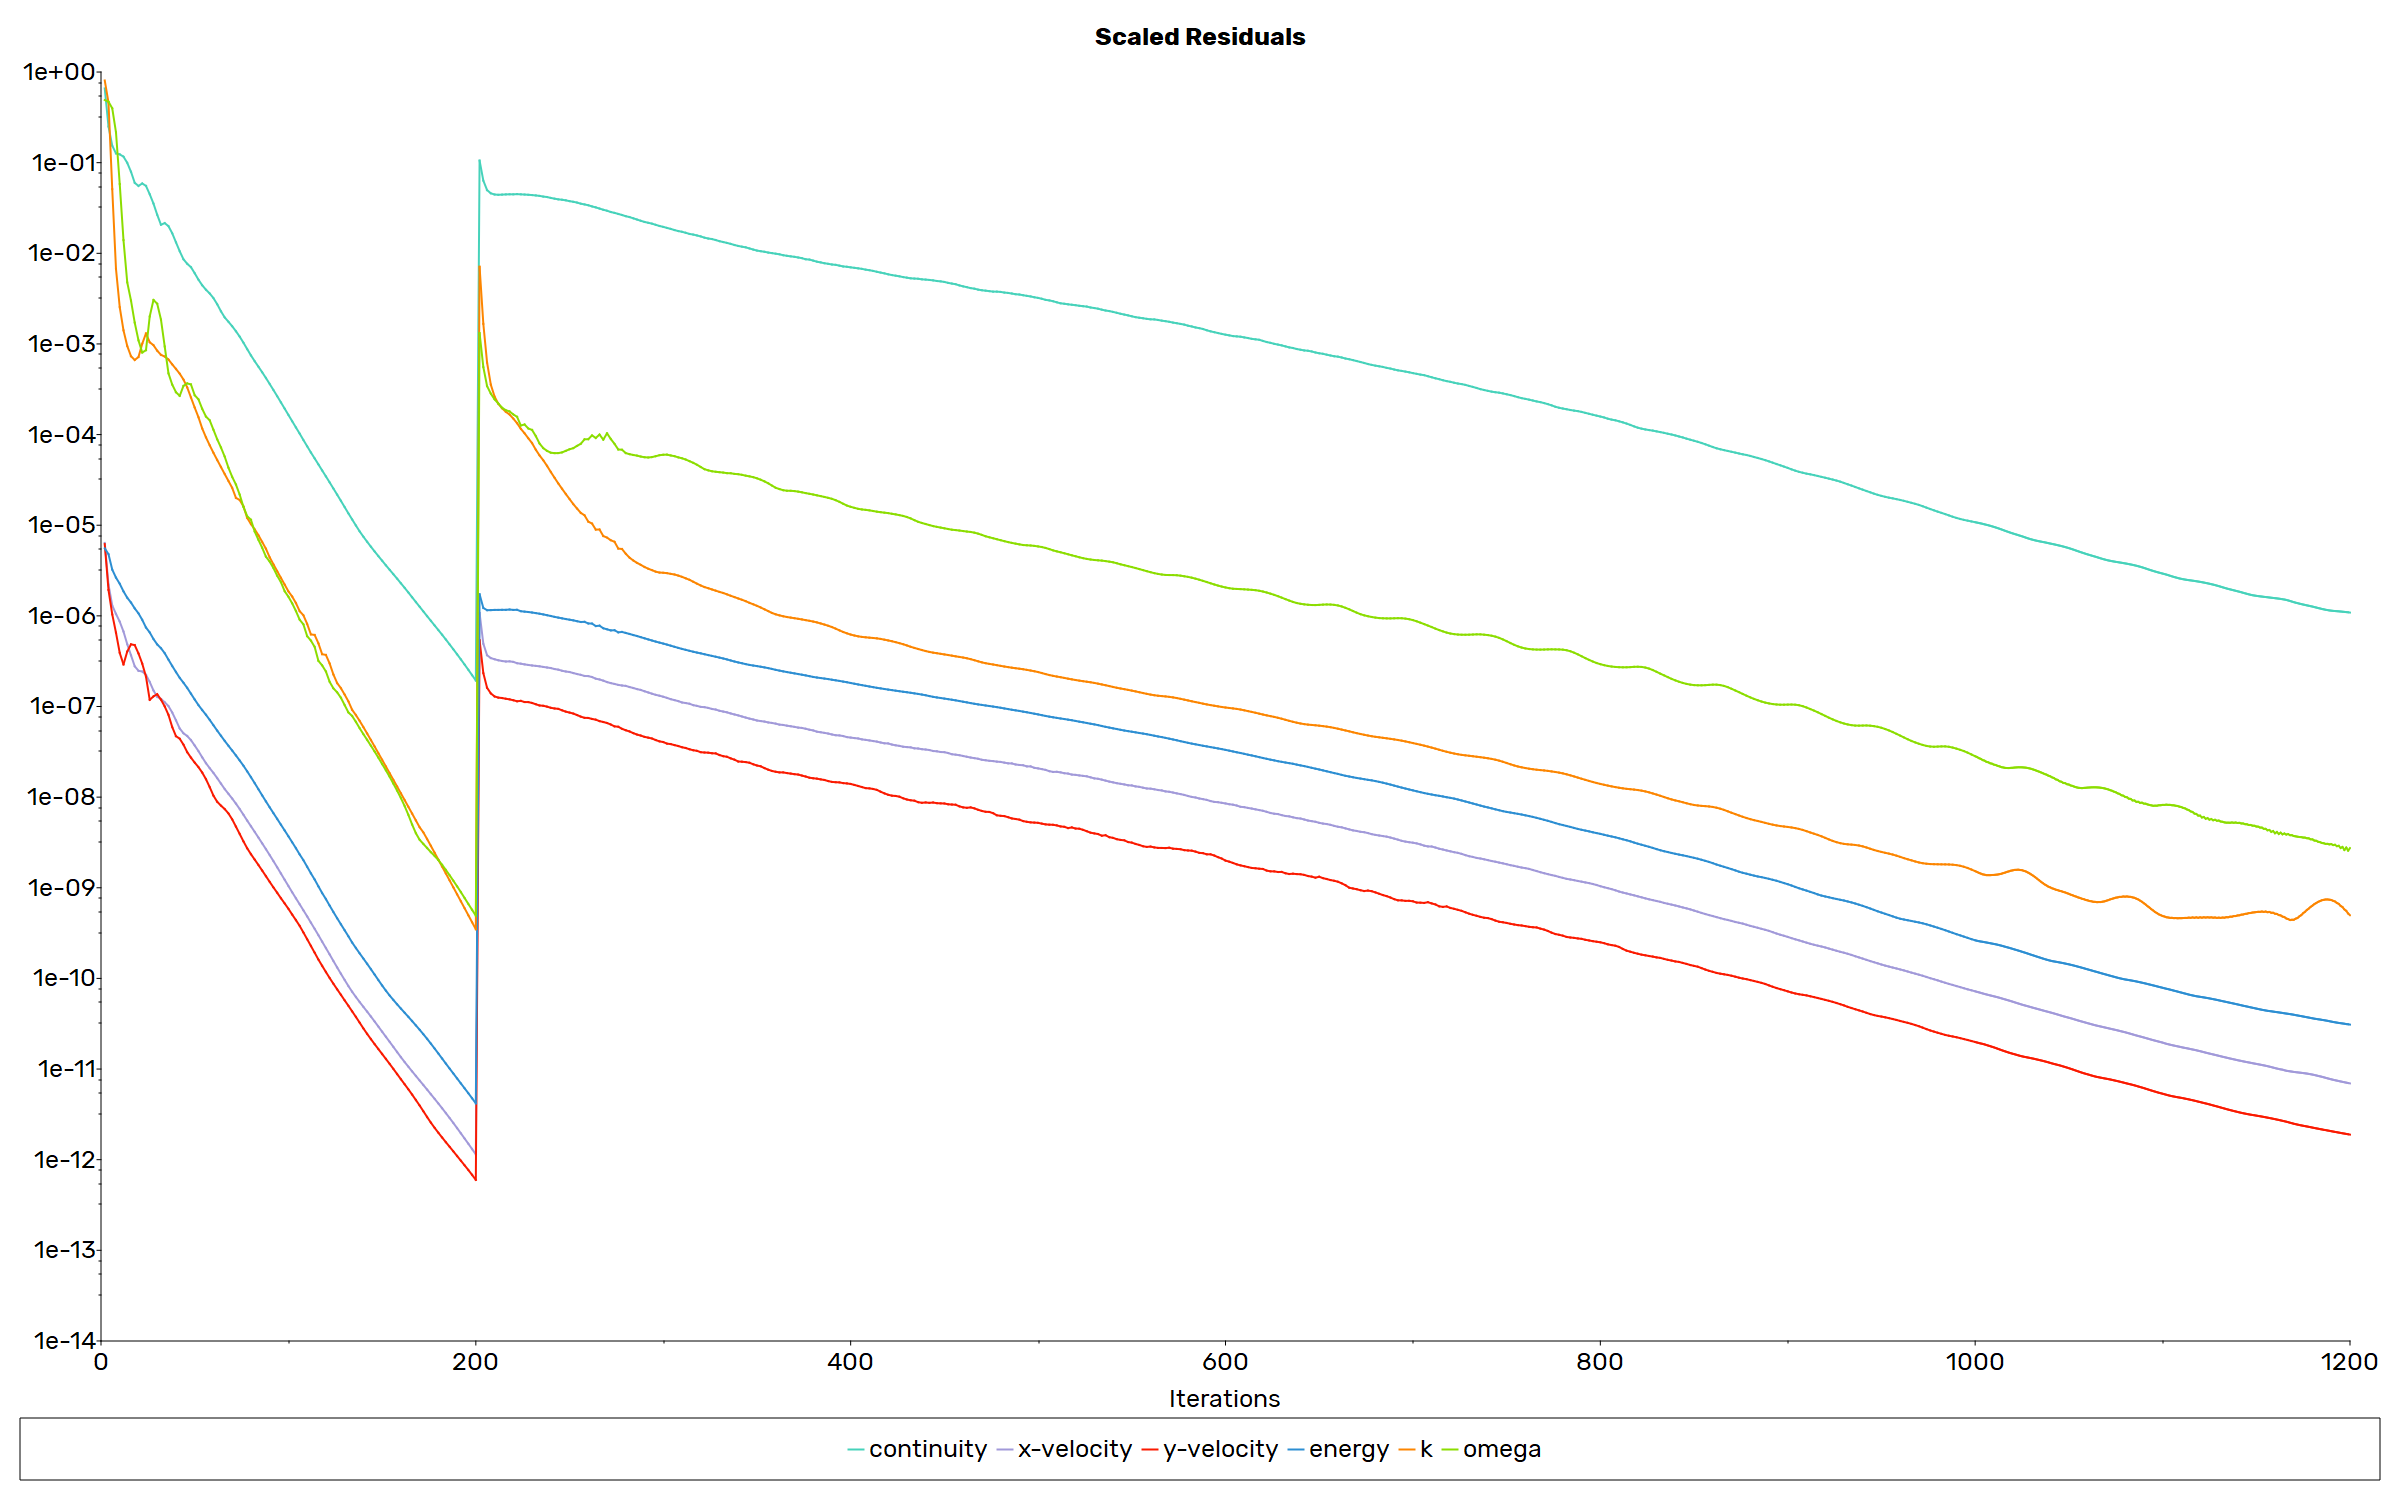
\includegraphics[width=\linewidth]{fluent_residuals_M0.95}
\caption{$M = 0.95$, pressure-based.}
\end{subfigure}
\caption{Scaled residuals from Fluent. At $M = 1.47$ they level off at $10^{-4}$--$3\cdot10^{-3}$
while $C_D$ is already constant (Figure~\ref{fig:history}a), which is why convergence is judged on
$C_D$.}
\label{fig:residuals}
\end{figure}
